% for sharelatex https://www.sharelatex.com/github/
% !TEX program = pdflatex

\documentclass{amsart}

\usepackage{amsmath}
\usepackage{amssymb}
\usepackage{cite}
\usepackage{graphicx}
\usepackage{url}
\usepackage{color}
\usepackage[notref,notcite]{showkeys}

\newtheorem{theorem}{Theorem}
\newtheorem{lemma}{Lemma}
\newtheorem{corollary}{Corollary}
\newtheorem{proposition}{Proposition}
\newtheorem{example}{Example}
\newtheorem{definition}{Definition}
\newtheorem{observation}{Observation}

\newcommand{\RR}{\mathbb R}
\newcommand{\ZZ}{\mathbb Z}
\newcommand{\fS}{\mathfrak S}

\newcommand{\aut}{\mathcal A}
\newcommand{\pairing}{\mu}
\newcommand{\tree}{\mathsf{T}}
\newcommand{\shape}{\mathsf{S}}
\newcommand{\ptangle}{\mathsf{X}}
\newcommand{\tangle}{\mathsf{Y}}
\newcommand{\ltangle}{\mathsf{L}}
\newcommand{\id}{\iota}
\newcommand{\wrtwo}{\wr \ZZ_2}

% arxivness
\newcommand{\arxiv}[1]{#1}
\newcommand{\notarxiv}[1]{}

% notes
\definecolor{violet}{rgb}{0.730,0.555,0.769}
\definecolor{purple}{rgb}{0.459,0.109,0.538}
\definecolor{grey}{rgb}{0.4,0.4,0.4}
\newcommand{\EM}[1]{\colorbox{violet}{\textcolor{white}{Erick: #1}}}

\newcommand{\FIGspr}{\
\label{FIGspr}
\begin{figure}
  \arxiv{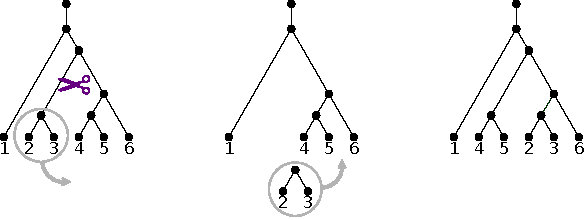
\includegraphics[width=4in]{figures/spr-definition}}
\caption{\
  A subtree-prune-regraft move.
}
\end{figure}
}

\newcommand{\FIGtanglegram}{\
\label{FIGtanglegram}
\begin{figure}
  \arxiv{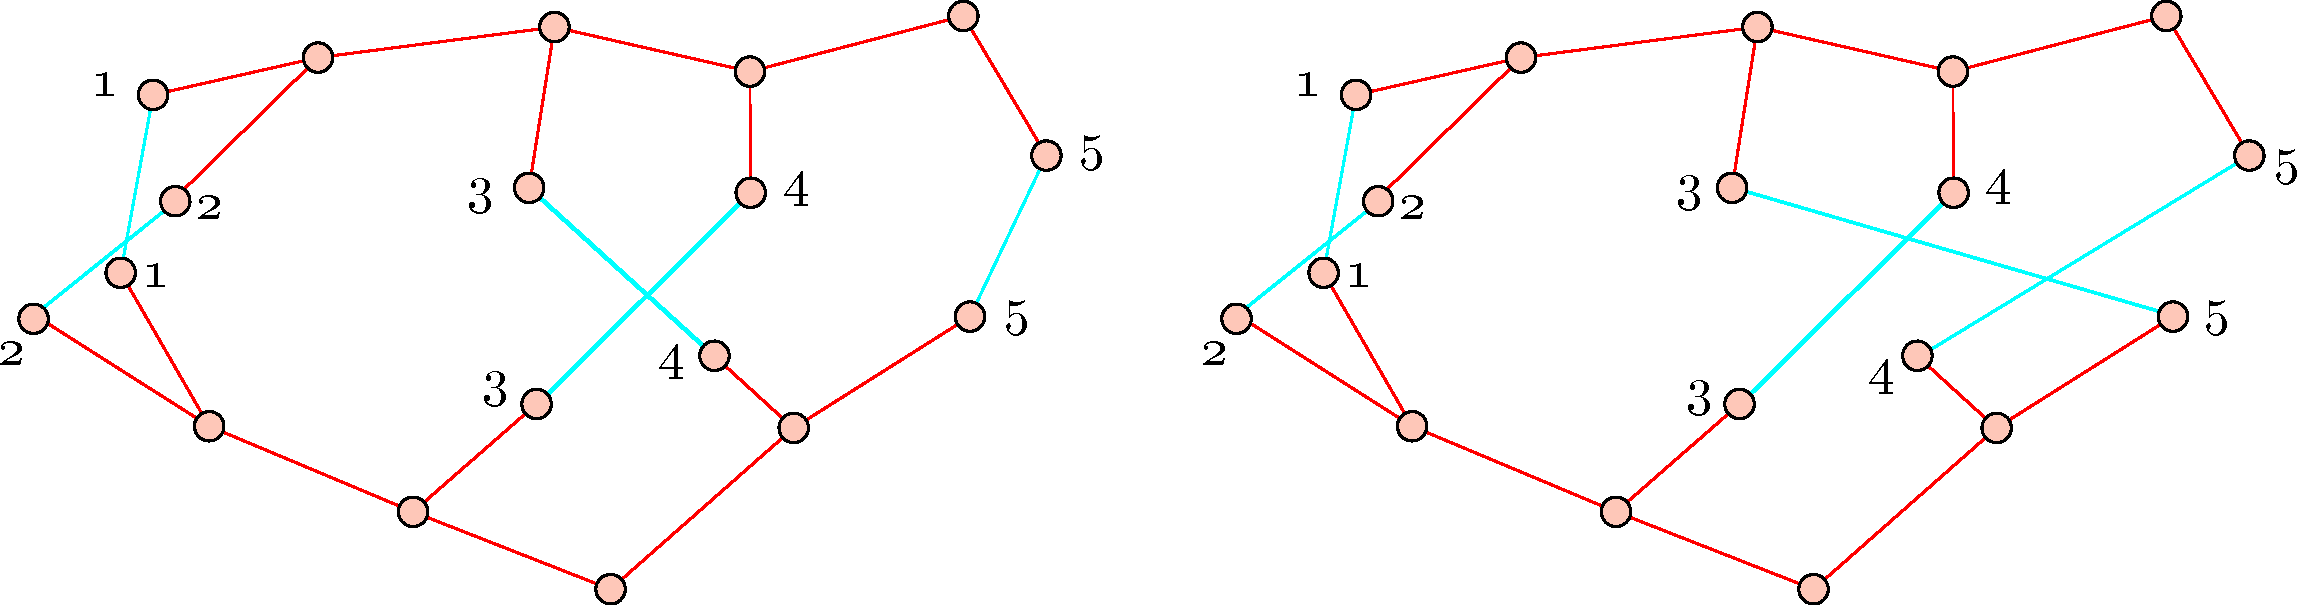
\includegraphics[width=5in]{figures/alternate-labeling}}
\caption{\
  Two equivalent labelings of the same tanglegram.
  Alternatively, they can be thought of as two permutations that are equivalent after taking symmetries of the bottom tree into account, or more formally two elements of the symmetric group which are equivalent under the action of the leaf automorphism group of the bottom tree.
}
\end{figure}
}

\newcommand{\FIGcountSymm}{\
\label{FIGcountSymm}
\begin{figure}
  \arxiv{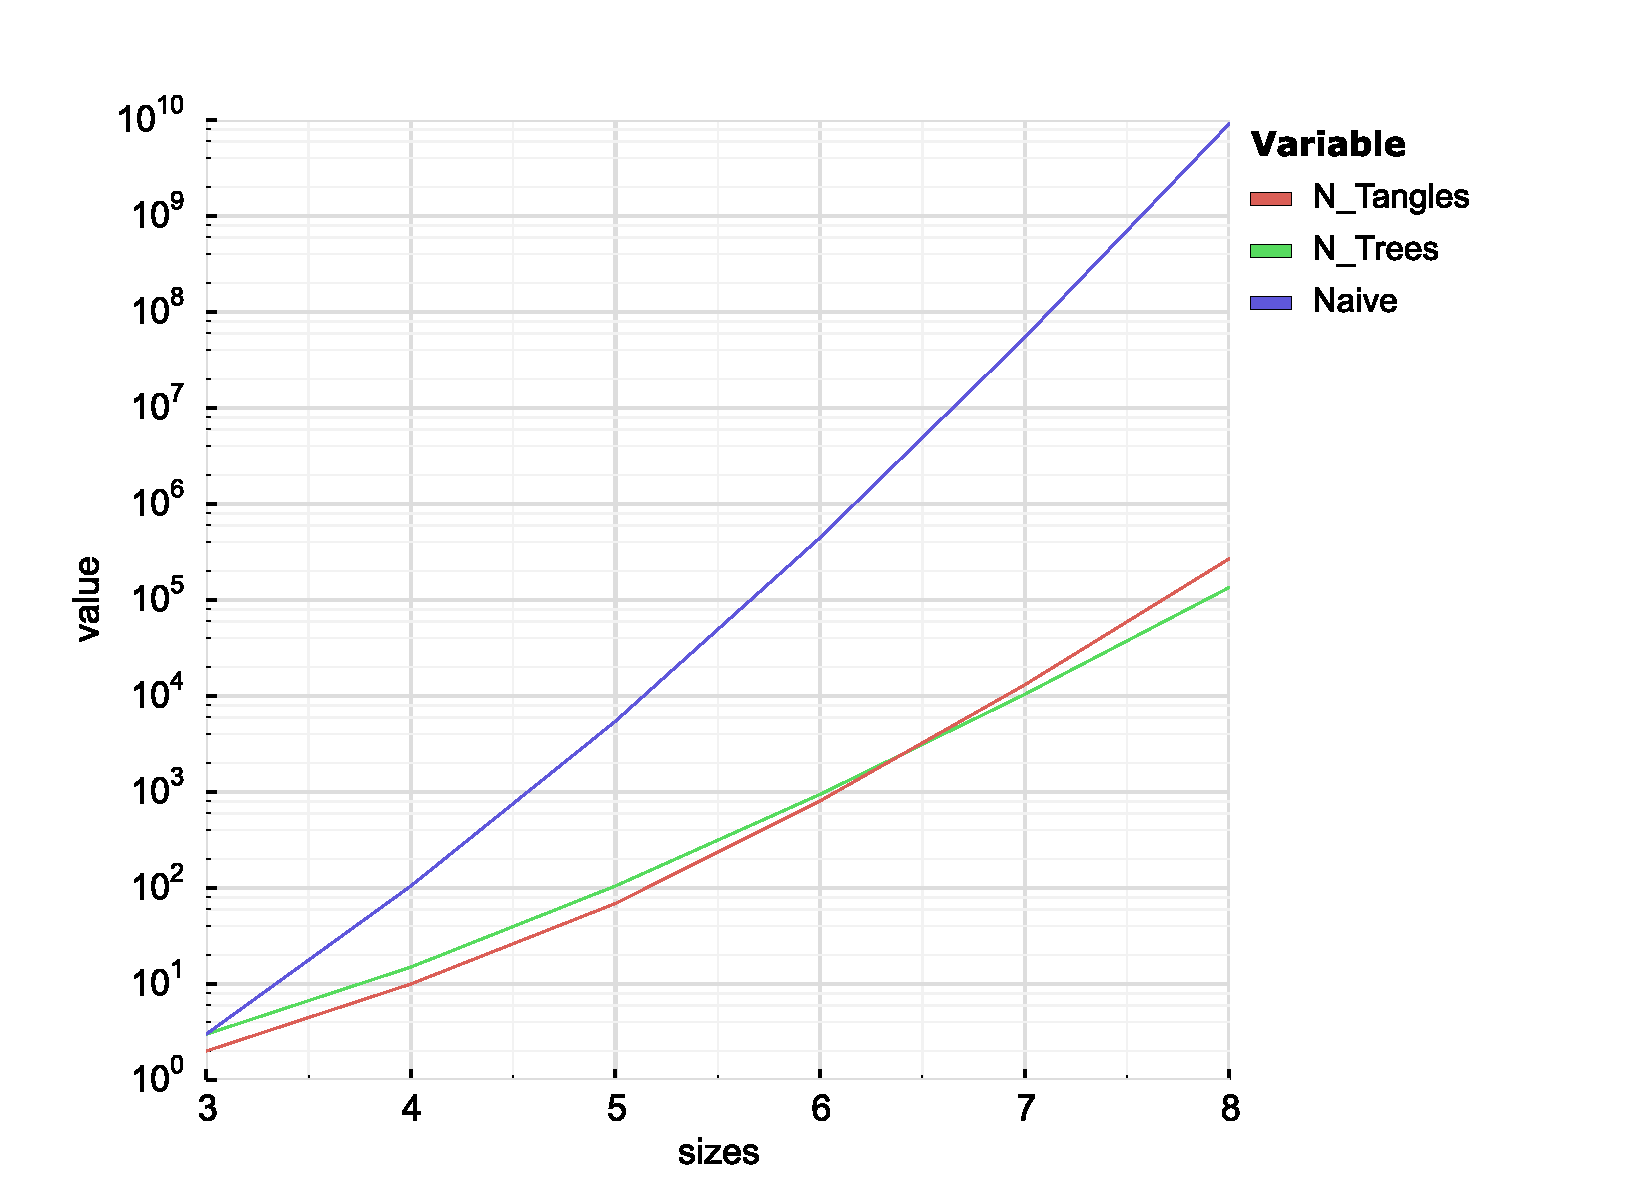
\includegraphics[width=.8\linewidth]{figures/symmetric-count}}
  \caption{Counts of stanglegrams compared to the naive count of stanglegrams.}
\end{figure}
}

\newcommand{\FIGcountAsymm}{\
\label{FIGcountAsymm}
\begin{figure}
  \arxiv{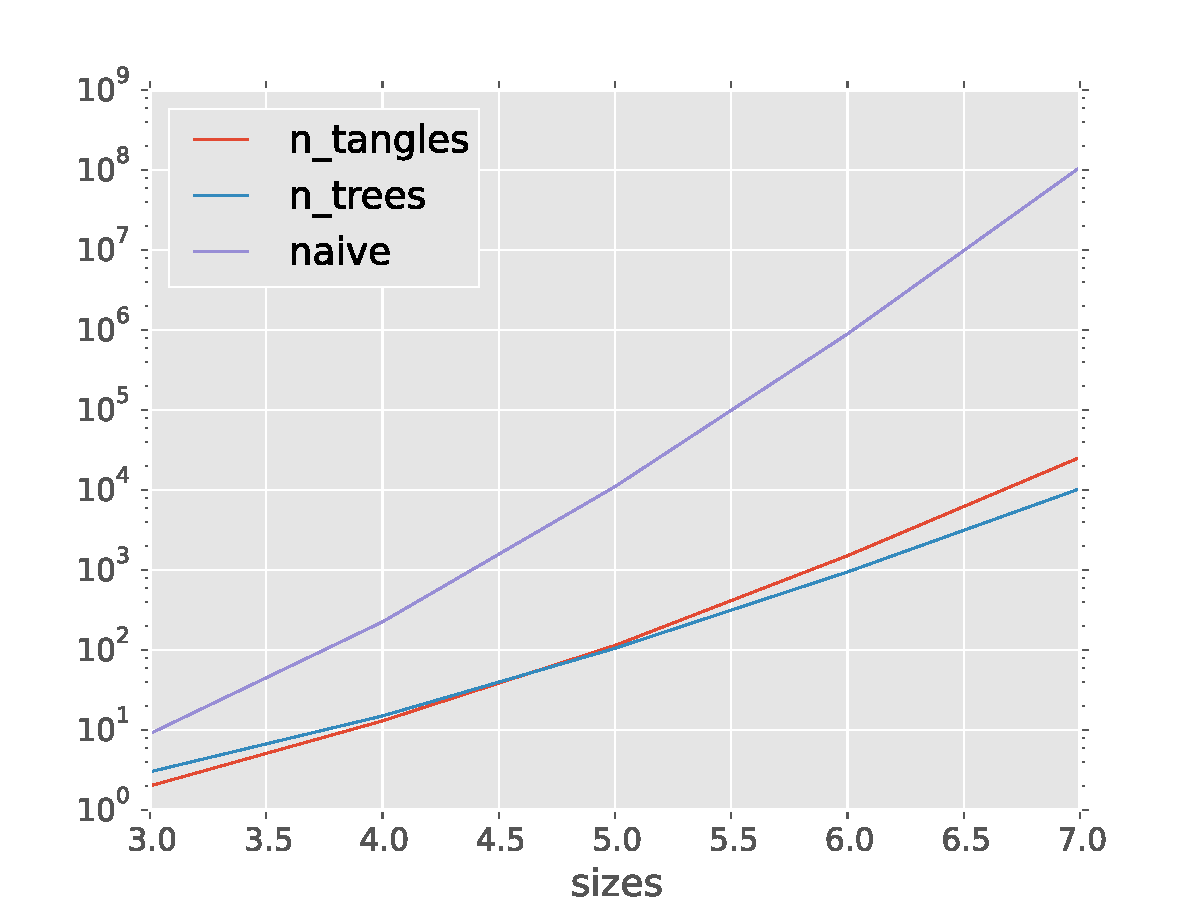
\includegraphics[width=.8\linewidth]{figures/asymmetric-count}}
  \caption{Counts of tanglegrams compared to the naive count of tanglegrams.}
\end{figure}
}


\begin{document}
\title{Enumerating rooted tanglegrams}
\author[Matsen]{Frederick A. Matsen IV}
\address{Fred Hutchinson Cancer Research Center \\ Seattle, WA}
\thanks{Research supported in part by National Science Foundation award 1223057 and National Institutes of Health grant R01 GM113246-01}


\date{\today}

\begin{abstract}
Many interesting discrete mathematics problems concerning phylogenetic trees are defined in terms of the relative labeling of pairs of rooted leaf-labeled trees.
These relative labelings are naturally formalized as so-called ``tanglegrams.''
Although there has been considerable work on planar embeddings of tanglegrams, their symmetries have not yet been explored.
Understanding symmetries of tanglegrams would help enumerate the distinct problems on relatively labeled pairs of trees, enable amortized algorithms, and reveal natural symmetries of spaces associated with such problems.
In this paper we develop methods to enumerate tanglegrams up to isomorphism, and we investigate the representation of the symmetric group induced by its action on tanglegrams.
\end{abstract}

\maketitle


\section{Introduction}
As a motivating example, we consider the problem of computing the \emph{subtree-prune-regraft} (SPR) distance between two leaf-labeled phylogenetic trees.
An SPR move cuts one edge of the tree and then reattaches the resulting rooted subtree at another edge (Figure~\ref{FIGspr}).
The SPR distance between two (phylogenetic, meaning leaf-labeled) trees $t_1$ and $t_2$ is the minimum number of SPR moves required to transform $t_1$ into $t_2$.
\FIGspr

Let's say that we wanted to calculate the SPR distance between every pair of trees.
Na\"ively this would require the binomial coefficient given by the number of phylogenetic trees choose two.
However, the distance between two such trees does not depend on the actual labels of $\ell_1$ and $\ell_2$, so one can permute the numerical labels of the leaf nodes, which would result in the same distance if the permutation was applied identically on both the starting and ending trees (and trees on the shortest SPR path between the two).
Furthermore, a path made by SPR moves made by intermediate trees between the two trees could also have its labels permuted in order to give a path between the trees with permuted leaf labels.
Thus, problems like SPR distance do not concern the actual leaf labels as such, but rather use the leaf labels as markers that can be used to map leaves of one phylogenetic tree on to another.
The problem and its solutions are actually defined in terms of a \emph{relative} leaf labeling.

Such discrete mathematics problems and objects defined in terms of pairs of labeled combinatorial objects are ubiquitous in computational biology.
In addition to SPR distances and their cousin distances formed by \emph{nearest-neighbor-interchange} and \emph{tree bisection and reattachment} \cite{wiki:treeRearrangement}, we have their corresponding biological questions concerning ``supertree'' reconstruction \cite{Whidden2014-ku} and reconciliation of gene transfer networks \cite{Boon2013-mc}.
Because such moves are used in both maximum-likelihood heuristic search and Bayesian Markov chain Monte Carlo (MCMC) tree reconstruction, the geometry of phylogenetic trees under such moves has substantial consequences in terms of phylogenetic tree reconstruction \cite{Whidden2014-yt}, and tanglegrams induce natural symmetries of pairs of points in these spaces.

Another line of inquiry in computational biology concerns species delimitation, which can naturally be phrased in terms of inference of a partition of labeled objects.
In an analogous way, scientists use MCMC to explore the posterior on such partitions \cite{Yang2010-kc}, and comparison of the results can be performed using distances between the partitions via distances such as \cite{Gusfield2002-il}.
These partitions can also be thought of as a certain type of leaf-labeled tree of height two (see description below), and thus they also form a problem concerning relative leaf labeling of phylogenetic trees.

The concept of a pair of phylogenetic trees with a relative leaf labeling can be formalized as the graph-theoretic notion of a \emph{tanglegram} (Figure~\ref{FIGtanglegram}).
A tanglegram is a pair of trees on the same set of leaves with matching leaves in the two trees joined by an edge. \cite{Venkatachalam2010-zh}.
There has been extensive work on the problem of drawing tanglegrams minimizing crossings \cite{Buchin2008-lc,Lozano2008-tp,Bansal2009-ni,Bocker2009-xl,Fernau2010-an,Venkatachalam2010-zh}.
\FIGtanglegram

However, there has been almost no work enumerating or finding other properties of this object, which formalizes the notion of a relative leaf labeling of a pair of phylogenetic trees.
Described slightly more formally, one can consider the projections starting with ordered pairs of phylogenetic trees
\begin{equation}
\label{eq:projChain}
\tree_n \times \tree_n \xrightarrow{\pi_\tangle} \tangle_n \xrightarrow{\pi_\shape} \shape_n \times \shape_n
\end{equation}
where $\tree_n$ is the set of $n$-taxon phylogenetic trees, $\tangle_n$ is the set of tanglegrams, and $\shape_n$ is the set of phylogenetic tree shapes (i.e.\ trees without leaf labels).
Rephrasing the above, many problems (such as SPR calculation) which are commonly phrased in terms of $\tree_n \times \tree_n$ are actually constant on pre-images of elements of $\tangle_n$ and thus factor to a problem on $\tangle_n$.

In this paper we show that tanglegrams are in one to one correspondence with certain single and double cosets of the symmetric group, both for labeled and non-labeled tangles.
There are efficient algorithms coded in GAP \cite{GAP4} to enumerate such cosets, which we use and extend via the SAGE \cite{SteinJoyner2005} interface to GAP.
These algorithms are quite fast compared to simpler approaches such as checking graph isomorphism.
We explore the mapping of pairs of plane-embedded trees into the set of tanglegrams and explore the action of a symmetric subgroup on tanglegrams by considering pre-images $\pi_\shape^{-1}(s_1, s_2)$ of each element of $(s_1, s_2) \in \shape_n \times \shape_n$ under $\pi_\shape$.
% We can characterize the isomorphism classes in terms of the symmetries of the two phylogenetic trees they contain.
Furthermore, tanglegrams are equipped with a natural action of subgroups of the symmetric group on the leaf set, which we describe.
We will also be interested in symmetric tanglegrams, or \emph{stanglegrams}, in which the order of the two trees (or tree shapes) is forgotten.
This is formalized by replacing the Cartesian products in \eqref{eq:projChain} with symmetric products, and can be analyzed using extensions to the non-symmetric case.


\section{Preliminaries}

\subsection{Phylogenetic trees and tree shapes}
For this paper, ``trees'' are leaf labeled rooted phylogenetic trees.
``Tree shapes'' are graph theoretic rooted trees without leaf labels.
Newick format is a parenthetical format used to describe trees. E.g. the left hand tree in Figure~\ref{FIGspr} would be represented by $(1,((2,3),((4,5),6)))$.

It is helpful to give labels to the leaves of these tree shapes in order to describe bijections between them.
We will do so in terms of \emph{standardized} phylogenetic trees: one (leaf-labeled) phylogenetic tree $\{t_{(i)}\}_{i=1,\ldots,k}$ for each tree shape $s_i$.
We will assume that a standardization has been fixed for the rest of the paper, such that for any tree shape $s_i$ we use $t_{(i)}$ to describe its standardization.

% For any phylogenetic tree $t$ the \emph{standard permutation} is the permutation $\sigma \in \fS_n$ mapping the leaf labels of its standardized tree $t_{(i)}$ to those of $t$.
% Note that all standard permutations are fixed for all trees on $n$ taxa once we choose a set of standardized trees.


\subsection{Algebraic preliminaries}
Given a subgroup $J$ of a group $G$, the \emph{right coset} $Jg$ of $G$ is the set of elements of the form $\{jg \mid j \in J\}$;
given two subgroups $J$ and $K$ of $G$, the \emph{double coset} $JgK$ for some $g \in G$ is the set of elements $\{jgk \mid j \in J, k \in K\}$.

Symmetric group on $n$ elements denoted by $\fS_n$.
We will use cycle notation for elements of the symmetric group, such as $(1\ 2) (3\ 4)$, which can be distinguished from phylogenetic trees in Newick format \cite{wiki:newick} such as $((1,2),(3,4));$, because symmetric group elements will not have commas or a trailing semicolon.

The action of the symmetric group is by relabeling items, not by moving them about in a positional representation.
For example, the action of the element $(1\ 3)$ on the list of numbers $2, 1, 3$ is the list $2, 3, 1$, not $3, 1, 2$.
In order to conform to the convention used in GAP \cite{GAP4} and hence by SAGE \cite{SteinJoyner2005}, \emph{we will use the leftmost first convention of writing products in the symmetric group.}
Thus, in cycle notation, $(1\ 2) (1\ 3) = (1\ 2\ 3)$.
We will correspondingly consider groups as acting on the right, such that the action of $x.(\sigma \tau)$ is $(x.\sigma).\tau)$, such that composition of group actions is composition of the corresponding maps.

Wreath product.
Define in two special cases: wreath square and with Z2?


\subsection{Tree symmetries}
It will be useful to start by describing symmetries of phylogenetic trees.

Given a tree $t$ we will say that an element $\alpha \in \fS_n$ is $t$-invariant if applying $\alpha$ to the leaves of $t$ results in the same leaf-labeled tree.
\begin{definition}
Given a (rooted) phylogenetic tree $t$ on $n$ leaves, let $\aut(t) \subset \fS_n$ be its set of $t$-invariant elements, called its leaf automorphism group.
\end{definition}
The group multiplication of two elements of $\fS_n$ is equivalent to the composition of the two relabelings.
For example, both of the connected trees in Figure~\ref{FIGspr} have the automorphism group generated by the elements $(2\ 3)$ and $(4\ 5)$.
Because every tree has at least one subtree of size two, the automorphism group of every tree has at least the symmetry of exchanging the two leaves of that subtree.

The automorphism group for a tree $t$ can be built up recursively.
Assume $t$ has subtrees $a$ and $b$.
If $a$ and $b$ are isomorphic as unlabeled trees (and thus have isomorphic automorphism groups), the automorphism group of $t$ is the wreath product $\aut(a) \wr \aut(b) \cong \aut(a) \wr \aut(a)$.
If $a$ and $b$ are not isomorphic in this way, then $\aut(t)$ is the direct product $\aut(a) \times \aut(b)$.
Thus, the automorphism group for a complete binary tree of depth $d$ is the $d$-fold wreath product of the two element group $\ZZ_2$ of itself, and the automorphism group of non-complete binary trees are subgroups of this iterated wreath product.


\section{Tanglegrams}

% XXX are we going to assume a numbering of the shapes? The current notation would seem to indicate so.
% We could have standardization be a function, a choice map from shapes to trees.
% Use tilde?

\begin{definition}
\label{def:abstractTanglegram}
A rooted $n$-\emph{tanglegram} is an ordered triple $(s_1, s_2, \phi)$ consisting of two tree shapes $s_1$ and $s_2$ and a bijection $\phi$ from the leaves of $s_1$ to the leaves of $s_2$.
Let $\tangle_n$ denote the set of $n$-tanglegrams.
\end{definition}

Using the ``standardization'' ideas above we have an alternate definition of a tanglegram:
\begin{definition}
\label{def:tanglegram}
A rooted $n$-\emph{tanglegram} is an ordered triple $(s_1, s_2, \pairing)$ consisting of two tree shapes $s_1$ and $s_2$ and an element of the symmetric group $\pairing \in \fS_n$.
\end{definition}
Assuming a standardization, as we do, this definition is the same as that in Definition~\ref{def:abstractTanglegram}, where the bijection $\phi$ in the first definition results from a $\pairing$ by applying the $\pairing$ action to the leaf set of the corresponding standardized trees $t_{(1)}$ and $t_{(2)}$.

We now note that because of tree symmetries, many such $\pairing$s give the same tanglegram.
Specifically, if $\alpha_1 \in \aut(t_{(1)})$ and $\alpha_2 \in \aut(t_{(2)})$, then $(s_1, s_2, \pairing)$ and $(s_1, s_2, \alpha_1 \pairing \alpha_2)$ give the same tanglegram.

In order to obtain a complete enumeration of tanglegrams, one can then collect all triples $(t_1, t_2, C)$ where $t_1$ and $t_2$ are tree shapes and $C$ enumerates double cosets of the form $\aut(t_1) \pairing \aut(t_2)$.

There is a graph realization of a tanglegram where every leaf of $t_1$ is connected via an edge to the corresponding leaf of $t_2$ under the bijection $\phi$.
There is a clear 1-to-1 correspondence between tanglegrams under relabeling and their graph realization.
If the two trees are rooted, we assume that something is done to distinguish the root nodes from other nodes of the tree.
As described in the section on future work, the case of unrooted tanglegrams does not follow directly from an understanding of rooted tanglegrams, and we will limit ourselves to rooted tanglegrams for the purposes of this paper.
This notion of tanglegram corresponds to that found previously in the literature.

Note that our definition respects the order of $t_1$ and $t_2$ by considering $(t_1, t_2, \pairing)$ to be different than the tanglegram $(t_2, t_1, \pairing^{-1})$ when $t_1$ and $t_2$ are different graph theoretically.
We can also consider an symmetric tanglegram, or \emph{stanglegram}, by identifying them.


\subsection{Tanglegram enumeration}
In order to obtain a complete enumeration of tanglegrams, one can then collect all triples $(t_1, t_2, C)$ where $t_1$ and $t_2$ are tree shapes and $C$ is a double coset of the form $\aut(t_1) \pairing \aut(t_2)$.
The set of such double cosets does not appear to follow easily from any general theory, but double cosets can be enumerated efficiently by GAP \cite{GAP4}.

\FIGcountAsymm

Stanglegrams, i.e.\ symmetric tanglegrams as defined above, have further symmetries.
For these one can start by ordering the tree shapes and only taking tanglegrams where $t_1$ is smaller than or equal to $t_2$ in this ordering.
In cases where $t_1 = t_2 = t$, exchanging the roles of $t_1$ and $t_2$ shows that $(t, t, \mu)$ is equivalent to $(t, t, \mu^{-1})$, meaning that we only need to take one of these for our enumeration.

To take the extra symmetry induced by stanglegrams into account, I wrote some GAP code to look for tanglegrams that remained the same after inversion on the basis of representatives (which have an easily defined total order), which was necessary because a na\"ive $O(n^2)$ search on double cosets (for which a total order is not available in GAP, but see \cite{Hulpke2003-em}) was too slow.
There are lots of stanglegrams (Figure~\ref{FIGcountSymm}), but significantly fewer than the number of pairs of distinct phylogenetic trees.

\FIGcountSymm

\bibliographystyle{unsrt}
\bibliography{tangle}
\end{document}


\subsection{Action of the tree normalizers on tanglegrams}
Recall that the \emph{normalizer} $N_H(G)$ of a subgroup $H$ in $G$ is the subgroup of elements $g \in G$ such that $gHg^{-1} = H$.
For any tangle $y = (t_1, t_2, \pairing)$ and $\sigma \in N_{\aut(t_2)}(\fS_n)$, there is an element $\rho_\sigma(y) \in \tangle_n$ induced by multiplication on the right by $\sigma$.
That is, for $\sigma \in \fS_n$ and $(t_1, t_2, \pairing) \in \tangle_n$,
\begin{equation}
\label{eq:action}
\rho_\sigma (t_1, t_2, \pairing) := (t_1, t_2, \pairing \sigma).
\end{equation}
This is well defined by the definition of the normalizer.
We can think about this as giving the leaf-to-leaf mapping obtained by reordering the \emph{image} of the pairing map, which are the leaves of $t_1$.
Identical considerations hold for a corresponding left map $\lambda_\sigma$.

Let $R(t)$ (resp.\ $L(t)$) be the set of tanglegrams $(t_1, t_2, C)$ such that $t_2$ (resp.\ $t_1$) is graph-theoretically isomorphic to $t$.
By the above, $N_{\aut(t)}(\fS_n)$ gives a well defined action on the right (resp.\ left) of $R(t)$ (resp.\ $L(t)$).
The normalizer criterion is in fact quite sensible from the perspective of phylogenetics, in that it ensures that pairs of sets of leaves that are images of each other under the automorphism group get the same treatment under the group action \eqref{eq:action} or its left map equivalent.

We also note that when $\sigma \in N_{\aut(t_2)}(\fS_n)$ as before,
\[
\rho_{\pairing^{-1} \sigma \pairing} (t_1, t_2, \pairing) =
(t_1, t_2, \sigma \pairing) =
\lambda_{\sigma} (t_1, t_2, \pairing).
\]

As an example of why \eqref{eq:action} is well defined for $\sigma \in N_{\aut(t_2)}(\fS_n)$ but not for all of $\fS_n$, let $t_1$ be the tree $((((1,2),3),4),5)$ and let $t_2$ be the tree $(1,(2,(3,(4,5))))$.
Abbreviating $\aut(t_i)$ with $A_i$, note that because $(4\ 5) \in A_2$, $A_1 e A_2$ and $A_1 (4\ 5) A_2$ are the same coset yet they have different images upon application of $(3\ 4)$:
\begin{align*}
A_1 (3\ 4) A_2 & = \langle (1 2) \rangle \{(3\ 4), (3\ 5\ 4)\} \\
A_1 (4\ 5) (3\ 4) A_2 & = \langle (1 2) \rangle \{(3\ 4), (3\ 4\ 5)\}.
\end{align*}
This sort of behavior is to be expected whenever a $g$ (here played by $(3\ 4)$) is not in the normalizer of $A_2$ in $\fS_n$, such that there is an $\alpha$ (here played by $(4\ 5)$) such that $g \alpha g^{-1}$ is not in $A_2$, and the effect of this conjugation is not absorbed by $A_1$.

[Following on this, perhaps a more general criterion could be devised, such that for any $\sigma$ and $a_2$ there exists a $a_1 \in A_1$ and $\tilde a_2 \in A_2$ such that $\pairing a_2 \sigma = a_1 \pairing \sigma \tilde a_2$?]


\section{Labeled tanglegrams}
\subsection{Labeled tanglegram symmetries}
We are also interested in properties of labeled tanglegrams, and follow a similar path through planar labeled tanglegrams to describe them.
Labeled tanglegrams on a set of $n$ leaves are equivalent to $\tree_n \times \tree_n$, i.e.\ ordered pairs of labeled trees.
Labeled planar $n$-tanglegrams with a given pair of tree shapes (i.e.\ elements of $\pi_\shape^{-1}(s_1, s_2)$ for some $s_1$ and $s_2$) are in one to one correspondence with pairs of permutations, in which we connect taxa with the same label to form a tanglegram.
\emph{Note that this focus on labels is different from that in the previous section, in which the focus was on the bijection between the leaves, and it will lead to a different set up in terms of group actions.}

Let us begin by assuming a planar tree shape $t_1$ on $n$ taxa.
The labelings of this planar tree shape are equivalent to permutations $\fS_n$, and the group composition law can be thought of as doing relabeling.
The automorphisms of this planar tree shape giving the same (non-planar) labeled phylogenetic tree can then be thought of as a subgroup $\aut(t_1)$ of $\fS_n$ as above which acts on the left of $\fS_n$.
In this way the (non-planar) labeled phylogenetic trees with the given shape are equivalent to the right cosets $A(t_1) \sigma$ for $\sigma \in \fS_n$.

Similarly, given two tree shapes, the planar labeled tanglegrams with those tree shapes are given by elements of the direct product $\fS_n \times \fS_n$.
Then the (non-planar) tanglegrams are again equivalent to the right cosets $(\aut(t_1), \aut(t_2)) (\sigma_1, \sigma_2)$ for $\sigma_1, \sigma_2 \in \fS_n$.
Indeed, each pair of labeled phylogenetic trees defines a labeled tangle just by connecting leaves with the same label.

In order to enumerate these objects it is convenient to use the notion of a \emph{wreath product} with the two-element group $\ZZ_2$.
Because we will only need this particular wreath product, I will just remind the reader of the definition in this special case.

Given a group $G$, the wreath product of $G$ with $\ZZ_2$, denoted $G \wrtwo$, can be described as the direct product $G \times G \times \ZZ_2$ with the following ``twisted'' multiplication table, where $\tau$ is the non-identity element of $\ZZ_2$:
\begin{align*}
(a, b, \id) (c, d, \id) & = (ac, bd, \id) \\
(a, b, \id) (c, d, \tau) & = (ac, bd, \tau) \\
(a, b, \tau) (c, d, \id) & = (ad, bc, \tau) \\
(a, b, \tau) (c, d, \tau) & = (ad, bc, \id).
\end{align*}

We will use this concept to enumerate labeled stanglegrams up to automorphism when the tree shapes are identical.
However, first we note that $G \wrtwo$ is equivalent to the planar tanglegrams which have means of distinguishing between the two trees, say with different colors for the edges of the two trees, but which we can flip upside down.
This flipping is formalized by the presence of $\tau$; the edge coloring allows us to see the difference between $(\sigma_1, \sigma_2, \tau)$ and $(\sigma_2, \sigma_1, \id)$.

The connection with the wreath product is as follows, using the interpretation of elements of $\fS_n$ as providing leaf relabelings.
Each triple $(\sigma_1, \sigma_2, \id)$ relabels $t_1$ and $t_2$ via $\sigma_1$ and $\sigma_2$, respectively, and $(\sigma_1, \sigma_2, \tau)$ does the same but then flips the tree, exchanging $t_1$ and $t_2$.
Flipping before relabeling with a pair of group elements effectively exchanges the order of the pair, which corresponds to the ``twisted'' product law in the wreath product.
These represent all of the symmetries of such a labeled tanglegram.

Because flipping the tree before relabeling doesn't do anything (recall that tree shapes are identical), the collection of edge colored tanglegrams is equivalent to the right cosets $\aut(t_1) \times \aut(t_2) \times \ZZ_2 \, (\sigma_1, \sigma_2, \id)$ for $\sigma_1, \sigma_2 \in \fS_n$.
Now, if we forget the difference between $t_1$ and $t_2$, in our analogy by removing colors from the edges, the set of tanglegrams is equivalent to double cosets
$\aut(t_1) \times \aut(t_2) \times \ZZ_2 \, (\sigma_1, \sigma_2, \id) \, {\id} \times {\id} \times \ZZ_2$ for $\sigma_1, \sigma_2 \in \fS_n$.


\subsection{Labeled tanglegram enumeration}
In order to enumerate the labeled tanglegrams in terms of the tanglegrams as thus defined, it is easy to define a map that corresponds to de-labeling a map.
Indeed, the map
\[
\aut(t_1) \times \aut(t_2) \times \ZZ_2 \, (\sigma_1, \sigma_2, \id) \mapsto \aut(t_1) \sigma_1 \sigma_2^{-1} \aut(t_2)
\]
from right cosets of $\fS_n \times \fS_n \times \id$ to double cosets of $\fS_n$ is well defined.
These double cosets of $\fS_n$ give exactly the mappings $\pairing$ defining the possible tanglegrams.
Thus, the pre-image of this map for a given tangle gives the possible labelings of that tangle.

In the case of stanglegrams when the trees have identical shapes, these objects are identified as elements of the wreath product $\fS_n \wrtwo$.
There is still a well-defined map of these objects to the collection of double cosets $\aut(t) \pairing \aut(t)$ which are unique up to inversion of $\pairing$.
As in the previous case, the pre-image of this map for a given stangle gives the possible labelings of that tangle.


\subsection{Planar tanglegram enumeration}

We can think about the forgetful map
\[
f_T: planar_n \rightarrow \tree_n
\]
mapping each (labeled) planar tree to its corresponding phylogenetic tree.
Thus $f_T^{-1}(t)$ are the planar embeddings of a tree, which are in one-to-one correspondence with the automorphism group $\aut(t)$.

\[
0 \rightarrow \aut(t) \rightarrow planar_n \rightarrow \tree_n \rightarrow \shape_n \rightarrow 0
\]


It is easier to describe mappings between trees embedded in the plane than trees in the abstract, and thus we introduce the notion of a \emph{planar} tanglegram.
This notion is a slight simplification of the notion of a \emph{drawing} used by previous authors \cite{Venkatachalam2010-zh} which will be convenient for our purposes.
We use the term \emph{planar embedding} as it is used in graph theory.
If not otherwise specified, ``isomorphic'' applied to trees refers to usual graph isomorphism rather than an isomorphism of embedded trees.

Let $\fS_n$ denote the symmetric group on $n$ items.
\begin{definition}
\label{def:ptanglegram}
A rooted (resp.\ unrooted) \emph{planar $n$-tanglegram} is an ordered triple $(p_1, p_2, \pairing)$ where $p_1$ and $p_2$ are rooted (resp.\ unrooted) trees with $n$ leaves embedded in the plane, and $\pairing \in \fS_n$ giving the bijection between the leaves.
Let $\ptangle_n$ denote the set of planar $n$-tanglegrams.
\end{definition}

Of course, there is also a well-defined planar graph realization for planar tanglegrams obtained by connecting leaves of planar trees $p_1$ and $p_2$ under $\pairing \in \fS_n$.

Given a planar tanglegram define the forgetful map $f: \ptangle_n \rightarrow \tangle_n$ by
\begin{equation}
\label{eq:forgetful}
(p_1, p_2, \sigma) \mapsto (t_1, t_2, \phi_\sigma).
\end{equation}
This map is surjective because any tanglegram can be embedded in the plane.
Furthermore, the pre-image of the forgetful map's algebraic component can be described in terms of double cosets:
\begin{proposition}
\label{prop:doubleCosets}
Let $(p_1, p_2, \sigma)$ be a planar embedding of an $n$-tanglegram $y$. Then
\[
\aut(p_1) \sigma \aut(p_2) = \{\tau \in \fS_n \mid f(p_1, p_2, \tau) = y\}.
\]
\end{proposition}
\begin{proof}
By definition of the automorphism group of a planar tree, $f(p_1, p_2, \tau) = y$ for any $\tau \in \aut(p_1) \sigma \aut(p_2)$.
Now take $\tau$ from $\{\tau \in \fS_n \mid f(p_1, p_2, \tau) = y\} \setminus \aut(p_1) \sigma \aut(p_2)$.
Thus $\sigma \not \in \aut(p_1) \tau \aut(p_2)$, which implies that $f(p_1, p_2, \tau) \neq y$, a contradiction.
\end{proof}


\section{Bounds}
Alternatively, one could enumerate trees (with repetition) by finding a labeled representative phylogenetic tree for every tree shape, then for every phylogenetic tree using the bijection defined by leaves with the same label.
This implies:
\begin{observation}
\label{obs:count}
The number of binary rooted $n$-tanglegrams is bounded above by the number of rooted binary phylogenetic tree shapes on $n$ leaves times the number of phylogenetic trees on $n$ leaves, and thus is asymptotically smaller than the number of pairs of rooted binary phylogenetic trees.
\end{observation}
Indeed, the number of tanglegrams is closer to the number of trees than the number of pairs of trees (Fig.~\ref{FIGcountAsymm}).




\section{Discussion and future work}
These considerations also lead to a graph-theoretic interpretation for problems defined as minimizing paths on graphs with trees as vertices, such as SPR.
For example, rather than considering SPR as shortest path calculation on a graph with trees as vertices and edges being SPR moves, one can think of it as happening on a graph formed by pairs of trees with edges connecting pairs of tree pairs that are identical after one SPR move on one of the trees.
The SPR distance distance then is the distance from a given vertex to a vertex composed of identical trees.
This graph has symmetries from relabeling all tree leaves.
The resulting quotient graph is a graph with vertices $\tangle_n$ obtained by applying $\pi_\tangle$.

Effect of tree rearrangements such as SPR.

Amortized algorithms.

Here we note that unrooted tanglegrams have further symmetries that do not follow directly from the considerations described here.
Given a rooted tanglegram, it is easy to define an unrooted tanglegram by placing a leaf on each root node and mapping one of these leaves to the other.
However, this is a many-to-one map because different rootings of the trees in the unrooted tanglegram may have different rooted tree topologies and thus will be distinct rooted tanglegrams.
Even when two rootings have the same topology, the corresponding rooted tanglegrams may be different:
the tanglegram
$$((1,(2,(3,(4,(5,6))))), (1,(2,(3,(4,(5,6))))), (2\ 4\ 3))$$
when rerooted at the edge leading to taxon 1 becomes
$$((((((1,2),3),4),5),6), (((((1,2),3),4),5),6), (2\ 4\ 3));$$
upon renumbering this becomes
$$((1,(2,(3,(4,(5,6))))), (1,(2,(3,(4,(5,6))))), (2\ 3\ 4))$$
which is not isomorphic to the original.
Thus, unrooted tanglegrams can be thought of as equivalence classes of rooted tanglegrams, but this equivalence does not appear trivial.


\section{Acknowledgements}
I would like to thank Michael Landis, Arnold Kas, Chris Whidden, and Bianca Viray.

Authors of SAGE and GAP4 software.
Alexander Hulpke

\bibliographystyle{unsrt}
\bibliography{tangle}


\notarxiv{
\section{Figure legends}
\FIGspr
\FIGtanglegram
\FIGcount
}
\end{document}


% It is now straightforward to enumerate tanglegrams on $n$ leaves.
% To start, one might obtain all of the possible $n$-tanglegrams as the set of all triples $(t_1, t_2, C)$ as per Observation~\ref{obs:cosetMap}.
% Consider two phylogenetic trees $\ell_1, \ell_2$ with representatives $s_{(1)}, s_{(2)}$ and standard permutations $\sigma_{(1)}$ and $\sigma_{(2)}$.
% The group element $\sigma_{(1)}^{-1} \, \sigma_{(2)}$ maps the leaves of $s_{(1)}$ to the leaves of $s_{(2)}$ that they correspond as in the $[\ell_1, \ell_2, \id]$ tanglegram, where $\id$ is the identity element
% Indeed, $\sigma_{(1)}^{-1}$ maps the leaves of $\ell_1$ to the corresponding leaves of $s_{(1)}$ and $\sigma_{(2)}$ maps the leaves of $\ell_2$ to the corresponding leaves of $s_{(2)}$.
% Thus the triple $(s_{(1)}, s_{(2)}, \aut(s_{(1)}) \sigma_{(1)}^{-1} \, \sigma_{(2)} \aut(s_{(1)}))$ is an alternate way of writing the tanglegram $[\ell_1, \ell_2, \id]$.
% Furthermore, one can take $\ell_1$ to be each of the standardized trees, so that $\sigma_1 = \id$, and $\ell_2$ to be all of the labeled trees such that $\sigma_2$ ranges over all of $\fS_n$.
% Furthermore, by moving relabeling into the element of the symmetric group, we can just limit ourselves to $[\ell_1, \ell_2, \pairing]$ where $\ell_2$ is also a standardized tree.
%
% Thus in order to obtain a complete enumeration of tanglegrams, one can enumerate double cosets of the form $\aut(t_1) \pairing \aut(t_2)$ for a given $t_1$ and $t_2$.
% The set of such double cosets does not appear to follow easily from any general theory, but double cosets can be enumerated efficiently by an algorithm in GAP \cite{GAP4}.


